%&latex
\documentclass[12pt]{article}
\usepackage{amsthm,amsmath}
\usepackage{graphicx,psfrag,epsf}
\usepackage{enumerate}
\usepackage{natbib}
\usepackage{url} % not crucial - just used below for the URL
\usepackage{amsthm,amsmath}
\usepackage[utf8]{inputenc}

%\pdfminorversion=4
% NOTE: To produce blinded version, replace "0" with "1" below.
\newcommand{\blind}{1}

% DON'T change margins - should be 1 inch all around.
\addtolength{\oddsidemargin}{-.5in}%
\addtolength{\evensidemargin}{-.5in}%
\addtolength{\textwidth}{1in}%
\addtolength{\textheight}{1.3in}%
\addtolength{\topmargin}{-.8in}%


\begin{document}

%\bibliographystyle{natbib}

\def\spacingset#1{\renewcommand{\baselinestretch}%
{#1}\small\normalsize} \spacingset{1}


%%%%%%%%%%%%%%%%%%%%%%%%%%%%%%%%%%%%%%%%%%%%%%%%%%%%%%%%%%%%%%%%%%%%%%%%%%%%%%

\if0\blind
{
  \title{\bf Promoting analysis reproducibility with accessibility: An example in evolutionary biology}
  \author{Luna L. Sanchez Reyes\thanks{
    The authors gratefully acknowledge "Sustaining the Open Tree of Life", NSF ABI No. 1759838, and ABI No. 1759846.}\hspace{.2cm}\\
    School of Natural Sciences, University of California, Merced\\
    and \\
    Emily Jane McTavish \\
    School of Natural Sciences, University of California, Merced}
  \maketitle
} \fi

\if1\blind
{
  \bigskip
  \bigskip
  \bigskip
  \begin{center}
    {\LARGE\bf Promoting analysis reproducibility with accessibility: An example in evolutionary biology}
\end{center}
  \medskip
} \fi

\bigskip
\begin{abstract}
Reproducibility is essential for scientific development. Efforts
to increase computational reproducibility have focused on increasing availability
of code and data. However, availability does not imply accessibility, and the latter
is infrequently addressed, even if it is key to achieve full workflow automatization
and reproducibility. Using an example in evolutionary biology, we identify factors
that have specifically affected accessibility in
the natural sciences, and ways researchers can address this to ensure reproducible
and automatic workflows.
The Open Tree of Life project (OpenTree) has developed a platform that facilitates
availability of results from evolutionary biology research. However, baseline
computational knowledge and skills required to
access scientific results are often not found among target users. While documentation
is available, it is often written using highly specialized language that is also
 inaccessible for the average target user.
We present a set of principles to generate documentation that improves accessibility
of code and documentation and present a tutorial were we apply those principles.



\end{abstract}

\noindent%
{\it Keywords:}  open science, education, R, phylogenetics, tutorials
\vfill

\newpage
\spacingset{1.45} % DON'T change the spacing!
\section{Introduction}
\label{sec:intro}

Reproducibility --the extent to which consistent results are obtained when a scientific
experiment is repeated (\cite{repdef2021})-- is a key aspect for the advancement
of science, as it constitutes a minimum standard to understand scientific results,
to determine their reliability and generality, and eventually to build more scientific
knowledge upon those results (\cite{king1995replication, peng2011reproducible, powers2019open}).
Reproducibility rates in the natural sciences are low (\cite{ioannidis2005most, prinz2011believe}),
prompting concerns about a reproducibility crisis in the field (\cite{baker2016reproducibility}).
The scientific community has united to incentivize cultural changes that will improve
reproducibility rates long term, such as transparency, availability, and workflow
automatization, to name a few (\cite{peng2015reproducibility}).
We argue that accesibility is a key aspect that must accompany availability (Box 1)
in order to achieve full workflow automatization and reproducibility.

\bigskip
\bigskip

\noindent\fbox{%
    \parbox{\textwidth}{%
    \textbf{Box 1.}
      Availability does not imply accessibility. One example we really like is the
      marshmallows in an office story.
      The marshmallow bags were there, availabe for anyone in the office to eat
      the marshmallows inside. But the marshmallows stayed there for days, weeks even.
      And it was not until someone opened the bag and put the marshmallows in a tray,
      that people started actually eating them. They were gone in a matter of hours.
      Code is not marshmallows. But the point is that by
      sharing your code and documenting it might not be enough for the general researcher
      to reproduce results. Researchers will certainly be able to eventually figure it out,
      but the time needed
      to do so might not be worthy for them, or might not be something they can invest
      in, even if it would be useful for them long term, the short term investment
      is too intense.
    }%
}
\bigskip

We focus on identifying factors that have specifically affected accessibility in
the natural sciences, and ways researchers can address it to ensure reproducible
and automatic workflows.
We use an example in evolutionary biology. This example focuses on understanding
the shared ancestry among organisms through evolutionary trees. These
trees provide the basis to study and understand biological processes
(\cite{dobzhansky1973nothing}). Hence, improving reproducibility and availability
of phylogenetic research is relevant for many aspects of biological research.
The Open Tree of Life project (OpenTree) has developed a platform that facilitates
availability of results from phylogenetic research, by standardizing and storing
phylogenetic data with the goal of synthesizing a single phylogenetic tree encompassing
all life (\cite{opentreeoflife2019synth}).
All data in OpenTree is open access and available programmatically through its many
Application Programming Interface (API) services (\cite{opentreeAPIs}).
Additionally, R packages (\cite{michonneau2016rotl}) and Python libraries
(\cite{mctavish2021opentree}) have been developed as wrappers for OpenTree API services
to make them available to a wider programming audience.
The R and Python OpenTree wrappers have been utilized by computer-literate individuals,
to seamlessly establish reproducible workflows to use and reuse expert phylogenetic
knowledge for biological research (\cite{sanchez2019datelife}) and education
(\cite{nguyen2020phylotastic, phylotasticedtools, galacticedtools}).

The OpenTree project demonstrates that efforts to increase reproducibility and availability have also increased the baseline required computational knowledge and skills in phylogenetic research.
These computational skills requirements are likely increasing across all natural sciences.
Computing is not traditionally a core skill taught to biologists and naturalists.
However, many students are now being trained in R as a statistics and data analysis environment.
In order for reproducible computational tools to be adopted for research, they need to be much more accessible to reseachers.
Data and code availability is a core requirement for reproducibility research (\cite{peng2011reproducible, sandve2013ten, powers2019open}).
However, the utility of data resources is limited by the technical challenges of accessing the data.
In order to motivate reproducible research, that gap needs to be bridged.
In this work we focus on improving accessibility of code examples and documentation.
In particular, we identify the necessity for documentation that is written down using language that is common to the target audience to facilitate examination, application, and adoption of code by the wider audience.

We present a set of principles to generate documentation that improves accessibility of code and documentation. We applied these principles to a series of tutorials and vignettes for the OpenTree project.

\section{Methods}
\label{sec:meth}
\subsection*{Identifying hurdles to accesibility}

Good primary documentation for code describes general usage of individual functions, the components and variables a function can take, and it should be accompanied with function usage examples on how to apply it.
As opposed to code, primary documentation is written in natural language (i.e., any known human language, e.g., English, Spanish, Chinese) and usually makes use of highly specialized computational jargon (computationally specific concepts, words, and phrases) as well as formal language, which often slows down or even obstructs examination, application, and adoption of code by external individuals.
Because primary documentation is considered a professional document, acceptance of the research by the scientific community could be reduced if a more informal language is used.
Secondary types of documentation, such as vignettes and tutorials, demonstrate additional cases of individual function usage, and describe analysis workflows in more detail, as well as function associations to generate a specific analysis and results. While secondary documentation has become more common practice, it is still often generated using highly specialized language.

\subsection*{Adressing hurdles to accesibility: the principles}

\subsubsection*{1. Demonstrate integration of function usage with motivating examples}

We examined available primary documentation for the OpenTree API R wrapper (the package `rotl`),
and designed a workflow that visits as many functions as possible, and demonstrate
uses commonly requested by OpenTree users that are not demonstrated elsewhere.
By framing the function workflow using highly requested uses, the documentation acquires a
narrative arc that is easier to follow and remember by users. This facilitates the translation
of functions to specfic use cases in biology.

For the tutorial demonstrated here, we used the commonly requested use case of obtaining
a phylogenetic tree for all lineages within a specific taxonomic rank.

\subsubsection*{2. Demonstrate errors and warnings thoroughly}

Primary documentation focuses on demonstrating usage function with examples that
work seamlessly, without errors. We argue that the opposite is needed to support
user adoption of reproducibile workflows: demonstrate examples that do not work
as expected and exemplify ways to address them (Figure \ref{fig:first}). We identify inputs that would give
a wide range of warnings and errors, focusing on demonstrating these cases. This
helps users to not be afraid of errors and warnings, but instead to use them to
their advantage.
We also identify effects of warnings and errors downstream of the workflow.

We identify ways to evaluate inputs to know if they will produce an error, and design
alternatives on what to do when faced with an error or warning, and demonstrate
these alternatives.
One of the most essential skills in programming is interpreting and moving forward
from errors.
Many finely honed tutorials do not trigger errors, which precludes helping students
to develop the tools to understand and address errors when they do encounter them,
as they inevitably will.

\begin{figure}
\begin{center}
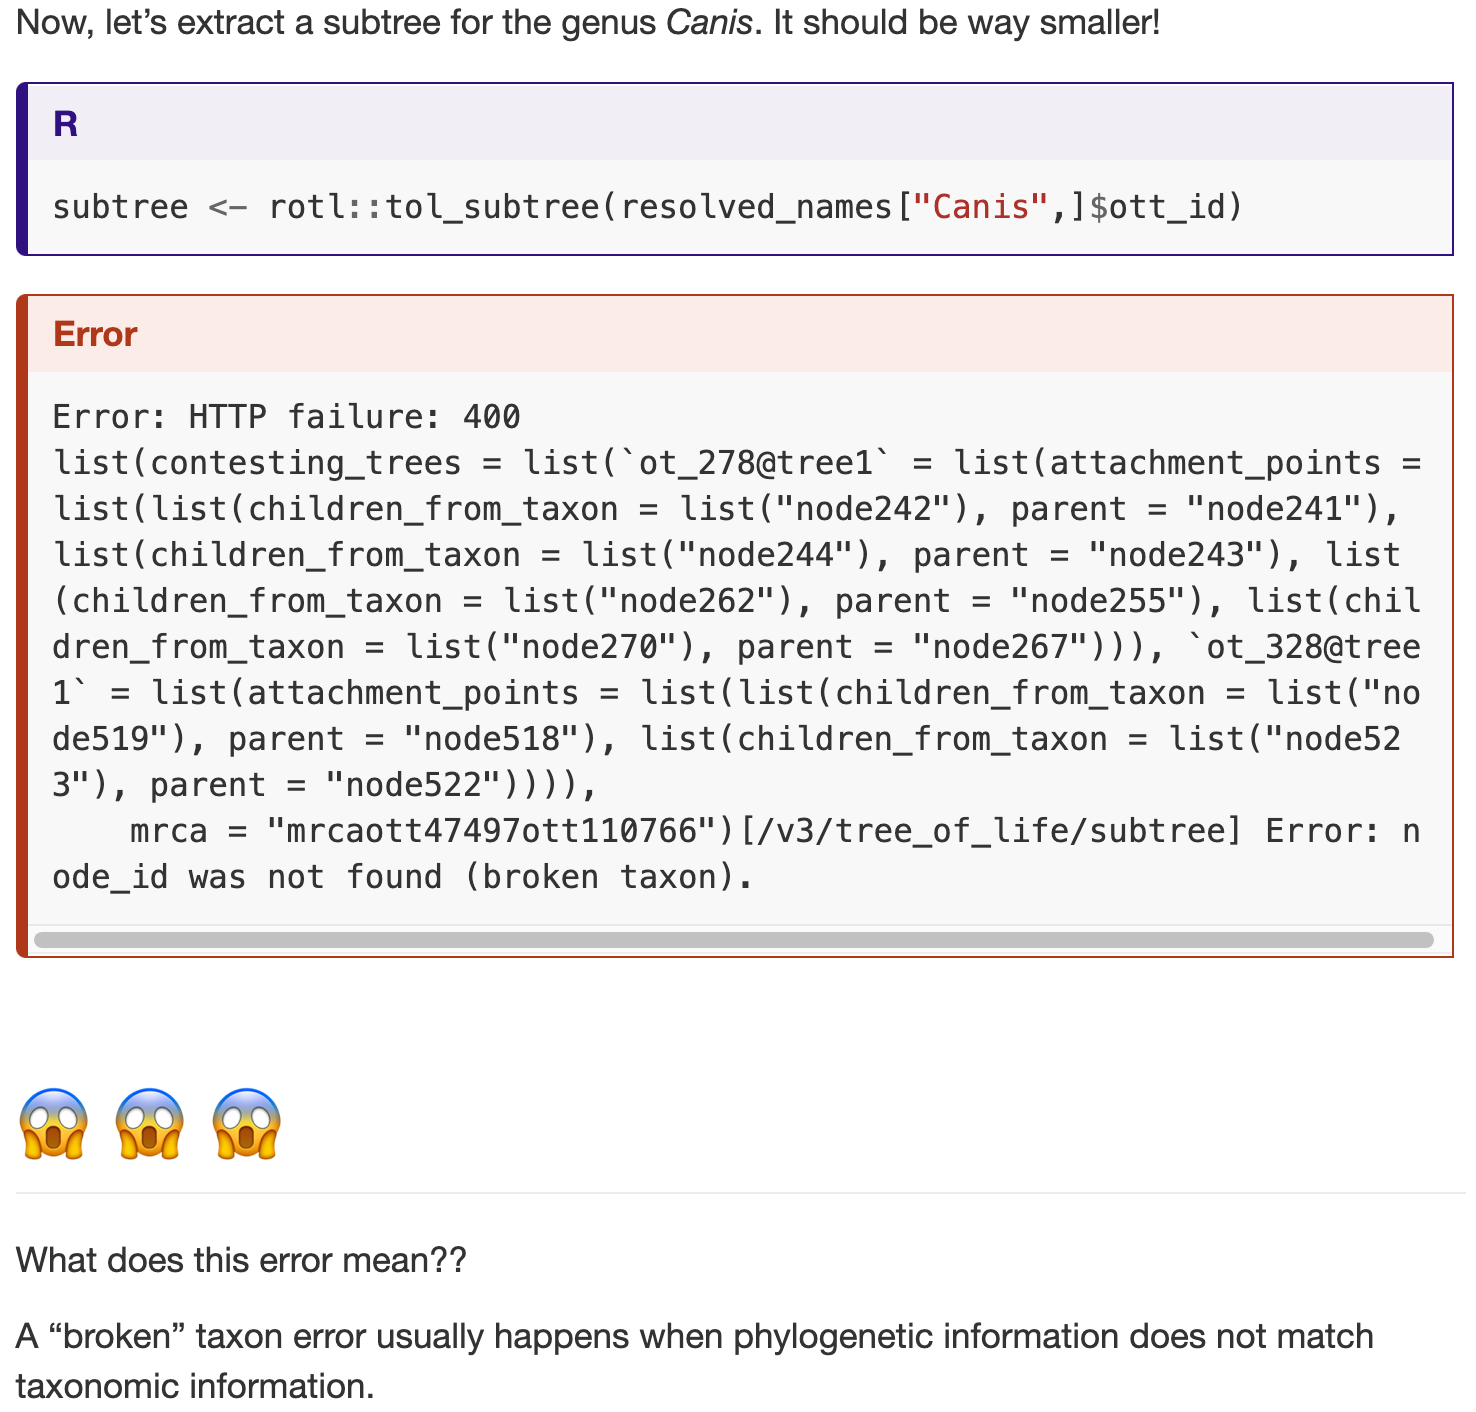
\includegraphics[width=3in]{fig1.png}
\end{center}
\caption{Snapshot of a section of the tutorial website, where we demonstrate a common error. \label{fig:first}}
\end{figure}

\subsubsection*{3. Avoid jargon and expert language}

Besides avoiding formal language, and incorporating elements of pop culture, such as picture
character icons known as "emojis", to make the language used more familiar to the
target audience (see Figure \ref{fig:first}), we made an effort to specifically
complement the primary documentation by identifying
computational concepts that were assumed or were not explained in depth.
We vetted the tutorials with an audience on workshops as well as individual user.
We choose examples that are charismatic for the audience.
For example, when we presented the tutorial for a team specialized in Amphibians,
we tailored the examples using frogs and their allies.


\subsubsection*{4. Make it stable through time}

We published the tutorials on a public, free license, free of cost, and free for
use and reuse repository and persistent website (\cite{RopentreeTutorials, RopentreeTutorialsWebsite}).
The tutorial is available for the users to go back to it any time they need it,
and to be passed on to other users (Figure \ref{fig:second}).

\begin{figure}
\begin{center}
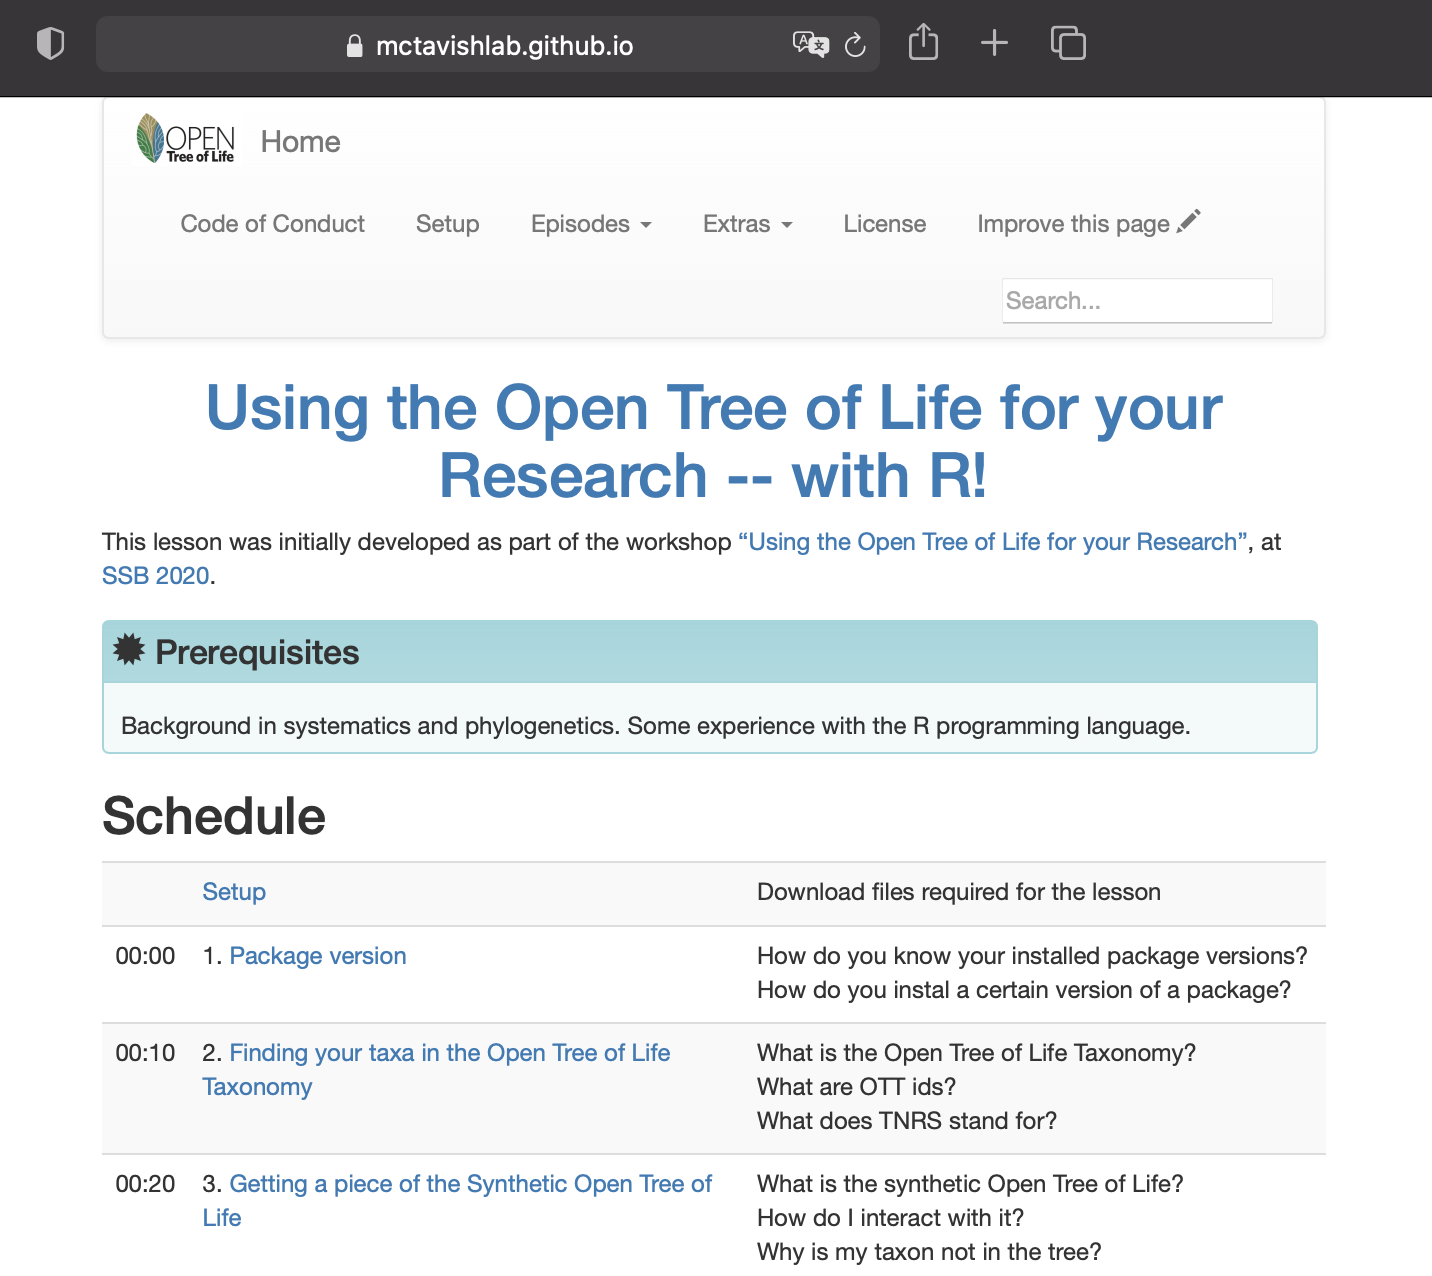
\includegraphics[width=3in]{fig2.png}
\end{center}
\caption{Snapshot of the home to our tutorial website, showing part of the schedule. \label{fig:second}}
\end{figure}

Following the carpentries, we created a main version of the tutorial that
is updated. Versions presented on workshops are a copy from the original repository,
and represent a stable and temporal snapshot of the functions and workflows presented
in the tutorial.

%%% \subsubsection*{5. The (now) classics of computational reproducibility}
%%%
%%% Provide all information on package version and system capabilities.
%%%
%%% > [name=Emily Jane McTavish]link to where/and how you did that

\section{Results and Discussion}
\label{sec:results}

We explain the warnings and errors and design ways to avoid them, and detect them beforehand (i.e., before using an input that would give an error). We explain the consequences of warnings.
We designed ways to access the different elements of the outputs.
We have received emails from senior researchers thanking us for this materials, and students have been able to engage using the packages with less hep from the PIs.

The principles to create tutorials described here facilitate adoption of software and analysis wokflows among researchers at different academic levels, from undergrads to established researchers.
It will also help closing the gap between students that had access to computational resources (and computational training) from an early age and students that did not. Late access to computational resources and training can occur due to lack of economic resources, often ocurring in households from underrepresented communities and minorites. It can also be due to gender-biased parental and community pressures, in which males are more often encouraged to perform activities related to computers, while females are discouraged.
How to balance software acceptance VS. adoption?
These principles can be used to aide not only reproducibility, but also software adoption in the natural sciences.
Discuss: why address accessibility and not other apects of reproducibility?


\section{Conclusion}
\label{sec:conc}

Making accessible reproducible workflows has several advantages:
save explanation/training time when analyses are run again by students and collaborators.
save research time for yourself when analyses are run again with more data, a different dataset, a different organism or biological model.
scientific efforts can build off of each other

\bigskip
\begin{center}
{\large\bf SUPPLEMENTARY MATERIAL}
\end{center}

\begin{description}

\item[Title:] Website and GitHub repository containing the complete teaching materials developed and demonstrated here.

\item[GitHub repository link:] \url{https://github.com/McTavishLab/R_OpenTree_tutorials}

\item[Website link:] \url{https://mctavishlab.github.io/R_OpenTree_tutorials}

\end{description}

\bibliographystyle{agsm}

\bibliography{Manuscript-bibliography}

\end{document}
